\chapter{Introduction} \label{introduction}

The APB4 GPIO Core is fully parameterised core designed to provide a
user-defined number of general purpose, bidirectional IO to a design.

The IO are accessible via an \emph{AMBA APB v2.0 Specification}
interface -- typically referred to as APB4 -- and the core operates
synchronously with the rising edge of the APB4 Bus Clock..

Inputs to the core may operate asynchronously to the core and will be
automatically synchronised to the bus clock. Outputs may be configured
to operate in push-pull mode or open-drain.

\begin{figure}[tbh]
	\centering
	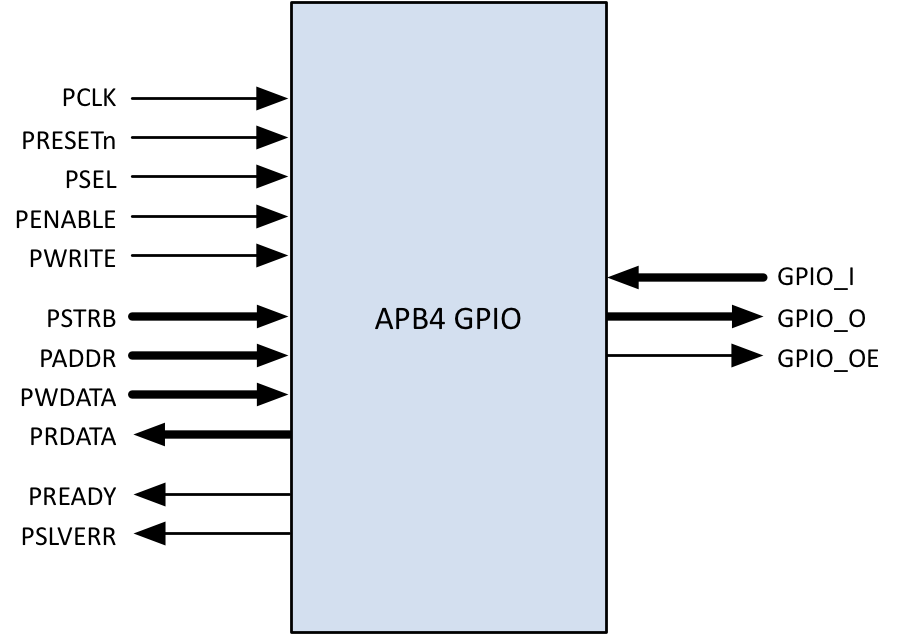
\includegraphics{assets/img/apb4-gpio-sig.png}
	\caption{APB4 GPIO Signalling}
	\label{fig:apb4-gpio-sig}
\end{figure}

\section{Features}\label{features}

\begin{itemize}
\item
  Compliant with AMBA APB v2.0 Specification
\item
  User-defined number of Bi-directional General Purpose IO
\item
  Automatic synchronisation of General Inputs to Bus Clock
\item
  Each General Output configurable as push-pull or open-drain
\end{itemize}